\chapter*{Cara Print NPM }

\par
Kita bisa melakukan print NPM dengan nomor satu per satu caranya sebagai berikut.


\begin{enumerate}
   

\item buka spyder dan ketikan kode seperti berikut
	\begin{figure} [h]
	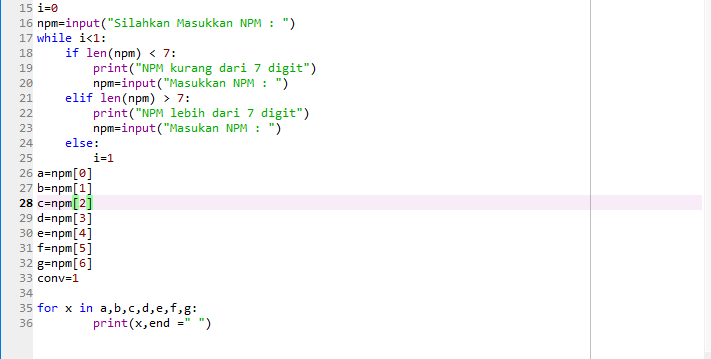
\includegraphics[width=10cm]{npm/npm3.png}
	\centering
	\end{figure}
	
	
	
 \item maka akan tercetak 
 \begin{figure} [h]
	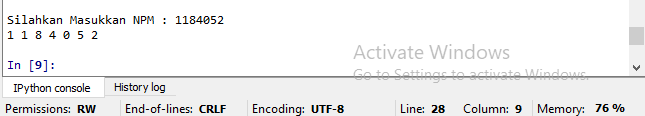
\includegraphics[width=9cm]{npm/npm4.png}
	\centering
	\end{figure}
 
	
	\end{enumerate}

